
\let\negmedspace\undefined
\let\negthickspace\undefined
\documentclass[journal,12pt,twocolumn]{IEEEtran}
\usepackage{cite}
\usepackage{amsmath,amssymb,amsfonts,amsthm}
\usepackage{algorithmic}
\usepackage{graphicx}
\usepackage{textcomp}
\usepackage{xcolor}
\usepackage{txfonts}
\usepackage{listings}
\usepackage{enumitem}
\usepackage{mathtools}
\usepackage{gensymb}
\usepackage[breaklinks=true]{hyperref}
\usepackage{tkz-euclide} 
\usepackage{listings}
\newtheorem{theorem}{Theorem}[section]
\newtheorem{problem}{Problem}
\newtheorem{proposition}{Proposition}[section]
\newtheorem{lemma}{Lemma}[section]
\newtheorem{corollary}[theorem]{Corollary}
\newtheorem{example}{Example}[section]
\newtheorem{definition}[problem]{Definition}
\newcommand{\BEQA}{\begin{eqnarray}}
\newcommand{\EEQA}{\end{eqnarray}}
\newcommand{\define}{\stackrel{\triangle}{=}}
\theoremstyle{remark}
\newtheorem{rem}{Remark}

%\bibliographystyle{ieeetr}
\begin{document}
%

\bibliographystyle{IEEEtran}


\vspace{3cm}

\title{
%	\logo{
Assignment-8
%	}
}
\author{EE22BTECH11012-A.Chhatrapati}


\maketitle

\newpage

%\tableofcontents

\bigskip

\renewcommand{\thefigure}{\theenumi}
\renewcommand{\thetable}{\theenumi}


\providecommand{\pr}[1]{\ensuremath{\Pr\left(#1\right)}}
\providecommand{\prt}[2]{\ensuremath{p_{#1}^{\left(#2\right)} }}        % own macro for this question
\providecommand{\qfunc}[1]{\ensuremath{Q\left(#1\right)}}
\providecommand{\sbrak}[1]{\ensuremath{{}\left[#1\right]}}
\providecommand{\lsbrak}[1]{\ensuremath{{}\left[#1\right.}}
\providecommand{\rsbrak}[1]{\ensuremath{{}\left.#1\right]}}
\providecommand{\brak}[1]{\ensuremath{\left(#1\right)}}
\providecommand{\lbrak}[1]{\ensuremath{\left(#1\right.}}
\providecommand{\rbrak}[1]{\ensuremath{\left.#1\right)}}
\providecommand{\cbrak}[1]{\ensuremath{\left\{#1\right\}}}
\providecommand{\lcbrak}[1]{\ensuremath{\left\{#1\right.}}
\providecommand{\rcbrak}[1]{\ensuremath{\left.#1\right\}}}
\newcommand{\sgn}{\mathop{\mathrm{sgn}}}
\providecommand{\abs}[1]{\left\vert#1\right\vert}
\providecommand{\res}[1]{\Res\displaylimits_{#1}} 
\providecommand{\norm}[1]{\left\lVert#1\right\rVert}
%\providecommand{\norm}[1]{\lVert#1\rVert}
\providecommand{\mtx}[1]{\mathbf{#1}}
\providecommand{\mean}[1]{E\left[ #1 \right]}
\providecommand{\cond}[2]{#1\middle|#2}
\providecommand{\fourier}{\overset{\mathcal{F}}{ \rightleftharpoons}}
\newenvironment{amatrix}[1]{%
  \left(\begin{array}{@{}*{#1}{c}|c@{}}
}{%
  \end{array}\right)
}

\newcommand{\solution}{\noindent \textbf{Solution: }}
\newcommand{\cosec}{\,\text{cosec}\,}
\providecommand{\dec}[2]{\ensuremath{\overset{#1}{\underset{#2}{\gtrless}}}}
\newcommand{\myvec}[1]{\ensuremath{\begin{pmatrix}#1\end{pmatrix}}}
\newcommand{\mydet}[1]{\ensuremath{\begin{vmatrix}#1\end{vmatrix}}}
\newcommand{\myaugvec}[2]{\ensuremath{\begin{amatrix}{#1}#2\end{amatrix}}}
\providecommand{\rank}{\text{rank}}
\providecommand{\pr}[1]{\ensuremath{\Pr\left(#1\right)}}
\providecommand{\qfunc}[1]{\ensuremath{Q\left(#1\right)}}
	\newcommand*{\permcomb}[4][0mu]{{{}^{#3}\mkern#1#2_{#4}}}
\newcommand*{\perm}[1][-3mu]{\permcomb[#1]{P}}
\newcommand*{\comb}[1][-1mu]{\permcomb[#1]{C}}
\providecommand{\qfunc}[1]{\ensuremath{Q\left(#1\right)}}
\providecommand{\gauss}[2]{\mathcal{N}\ensuremath{\left(#1,#2\right)}}
\providecommand{\diff}[2]{\ensuremath{\frac{d{#1}}{d{#2}}}}
\providecommand{\myceil}[1]{\left \lceil #1 \right \rceil }
\newcommand\figref{Fig.~\ref}
\newcommand\tabref{Table~\ref}
\newcommand{\sinc}{\,\text{sinc}\,}
\newcommand{\rect}{\,\text{rect}\,}
\let\vec\mathbf

\textbf{Question 9.3.4)}In an examination, 20 questions of true-false type are asked. Suppose a student tosses
a fair coin to determine his answer to each question. If the coin falls heads, he answer
true; if it falls tails, he answer false. Find the probability that he answers at least 12
questions correctly.\\
\solution \\
\begin{table}[ht]
    \centering
    \caption{Random Variables}
    \label{table:random-variables-9.3.4}
\begin{tabular}{|c|c|c|}
\hline
Variable & Value & Description \\
\hline
$X$ & $0 \le X \le 20$ & Number of correct questions \\
\hline
\end{tabular} 
\end{table}\\
\textbf{Gaussian}\\
Here $n=20$ and $p=0.5$\\
The mean $\mu$ of $X$
\begin{align}
\mu &= n\times p\\
&= 10
\end{align}
The variance $\sigma^{2}$ of $X$
\begin{align}
\sigma^{2} &= n\times p \times \brak{1-p}\\
&= 5
\end{align}
Let
\begin{align}
Z &\approx \frac{X-\mu}{\sigma}
\end{align}
Here, Z is a random variable with $\gauss{0}{1}$ \\
Normal-Distribution $f\brak{x}$
\begin{align}
	f\brak{x} = \int_{x}^{\infty}\frac{1}{\sqrt{2\pi}} \times e^{-\frac{x^2}{2}}
\end{align}
The $Q$-function from the Normal-Distribution
\begin{align}
	\qfunc{x} &= \pr{Z>x}
\end{align}
Since
\begin{align}
X &\ge 12
\end{align}
\begin{enumerate}
\item With a 0.5 correction:
\begin{align}
\pr{X \ge 12} &= 1-\pr{X<11.5}\\
X&<11.5\\ 
\implies Z &< \frac{11.5-\mu}{\sigma}\\
Z &< \frac{1.5}{\sqrt{5}}\\
Z &< 0.67082\\
\pr{X \ge 12}&=1-\pr{Z < 0.67}
\end{align}
On compution,
\begin{align}
\pr{Z < 0.67}&=0.74883\\
\implies \pr{X \ge 12}&= 0.2511
\end{align}
\item Without correction:
\begin{align}
X &\ge 12\\
Z &\ge \frac{12-\mu}{\sigma}\\
Z &\ge \frac{2}{\sqrt{5}}\\
Z &\ge 0.894\\
\pr{X \ge 12}&=\pr{Z \ge 0.894}\\
&=0.1855
\end{align}
\end{enumerate}
\textbf{Binomial}
\begin{align}
\pr{X\ge12} &= 1 - \pr{X<12} \\
&= \sum_{k=12}^{20}\myvec{n\\k}p^k\brak{1-p}^{n-k} \\
&= 0.2517
\end{align}
The graph\\
\begin{figure}[h]
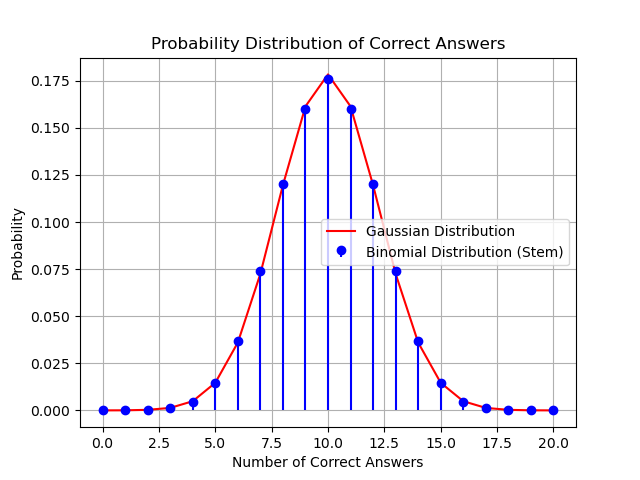
\includegraphics[width=\columnwidth]{./figs/dist.png}
\caption{Binomial vs guassian}
\label{fig:BvG_py}
\end{figure}
\end{document}
